\documentclass[aspectratio=169]{beamer}

% Minimal theme
\usetheme{default}
\usecolortheme{dove}

% Remove navigation symbols
\setbeamertemplate{navigation symbols}{}
\setbeamertemplate{footline}{%
  \hfill{\large\insertframenumber\,/\,\inserttotalframenumber}\hspace{0.8em}\vspace{0.5em}%
}

% Colors
\definecolor{popblue}{RGB}{52, 101, 164}
\definecolor{sampred}{RGB}{204, 0, 0}
\definecolor{paramgreen}{RGB}{0, 140, 70}
\definecolor{lightbg}{RGB}{245, 245, 250}
\definecolor{warnred}{RGB}{180, 40, 40}
\definecolor{orange1}{RGB}{220, 120, 0}
\definecolor{violet1}{RGB}{120, 50, 160}

\setbeamercolor{frametitle}{fg=popblue}
\setbeamercolor{title}{fg=popblue}

% Packages
\usepackage{pgfplots}
\usepackage{tikz}
\usetikzlibrary{shapes, arrows.meta, positioning, calc, decorations.pathreplacing, patterns, fit}
\pgfplotsset{compat=1.18}
\usepackage{amsmath, amssymb}
\usepackage{array}
\usepackage{fontenc}

\title{Long Context \& Efficient Attention}
\subtitle{Flash Attention $\cdot$ Sparse Patterns $\cdot$ KV Cache $\cdot$ State Space Models}
\date{}

\begin{document}

% ============================================================
% TITLE
% ============================================================
\begin{frame}
\titlepage
\end{frame}

% ============================================================
% THE QUADRATIC WALL
% ============================================================
\begin{frame}
\frametitle{The quadratic wall}

\begin{center}
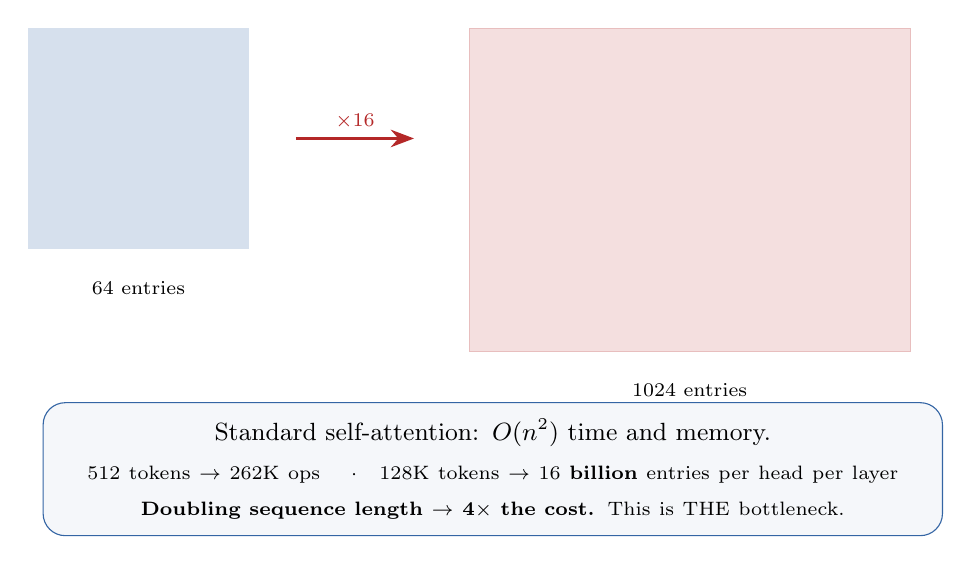
\begin{tikzpicture}
  % Small attention matrix
  \node[font=\small\bfseries, text=popblue] at (-4.5, 3) {$n = 8$};
  \draw[step=0.35, popblue!30, thin] (-5.4, 0.8) grid (-2.6, 3.6);
  \fill[popblue!20] (-5.4, 0.8) rectangle (-2.6, 3.6);
  \node[font=\scriptsize] at (-4, 0.3) {64 entries};

  % Arrow
  \draw[-Stealth, very thick, warnred] (-2, 2.2) -- (-0.5, 2.2);
  \node[font=\scriptsize, text=warnred, above] at (-1.25, 2.2) {$\times 16$};

  % Large attention matrix
  \node[font=\small\bfseries, text=warnred] at (3, 3) {$n = 32$};
  \fill[warnred!15] (0.2, -0.5) rectangle (5.8, 3.6);
  \draw[warnred!30, thin] (0.2, -0.5) rectangle (5.8, 3.6);
  \node[font=\scriptsize] at (3, -1) {1024 entries};

  % Formula
  \node[draw=popblue, fill=popblue!5, rounded corners=8pt, text width=11cm, align=center, inner sep=6pt, font=\small] at (0.5, -2) {
    Standard self-attention: $O(n^2)$ time and memory.\\[3pt]
    {\scriptsize 512 tokens $\to$ 262K ops \quad$\cdot$\quad 128K tokens $\to$ 16 \textbf{billion} entries per head per layer}\\[2pt]
    {\scriptsize \textbf{Doubling sequence length} $\to$ \textbf{4$\times$ the cost.} This is THE bottleneck.}
  };
\end{tikzpicture}
\end{center}
\end{frame}

% ============================================================
% WHY LONG CONTEXT MATTERS
% ============================================================
\begin{frame}
\frametitle{Why long context matters}

\begin{center}
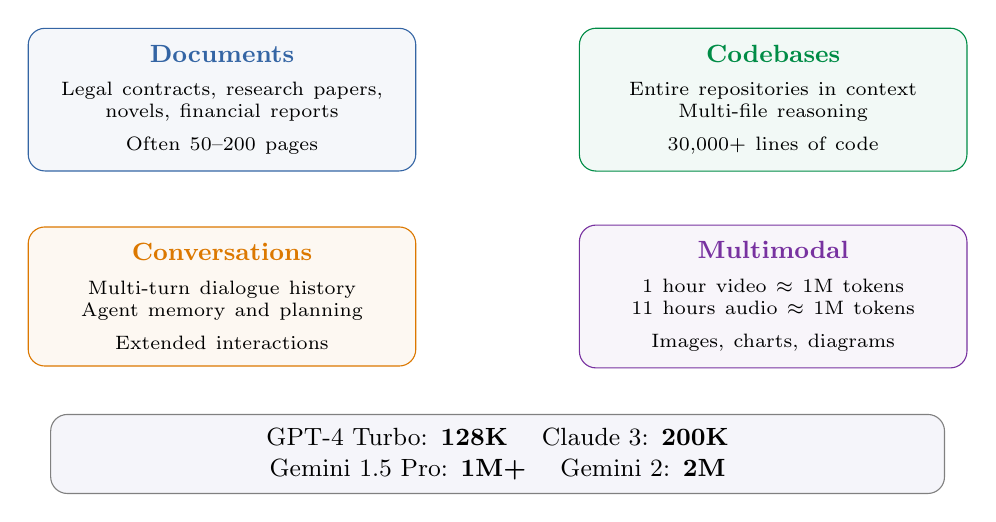
\begin{tikzpicture}
  % Use case cards
  \node[draw=popblue, fill=popblue!5, rounded corners=6pt, text width=4.5cm, align=center, inner sep=6pt] at (-3.5, 2) {
    {\small\bfseries\textcolor{popblue}{Documents}}\\[4pt]
    {\scriptsize Legal contracts, research papers,\\
    novels, financial reports\\
    Often 50--200 pages}
  };

  \node[draw=paramgreen, fill=paramgreen!5, rounded corners=6pt, text width=4.5cm, align=center, inner sep=6pt] at (3.5, 2) {
    {\small\bfseries\textcolor{paramgreen}{Codebases}}\\[4pt]
    {\scriptsize Entire repositories in context\\
    Multi-file reasoning\\
    30,000+ lines of code}
  };

  \node[draw=orange1, fill=orange1!5, rounded corners=6pt, text width=4.5cm, align=center, inner sep=6pt] at (-3.5, -0.5) {
    {\small\bfseries\textcolor{orange1}{Conversations}}\\[4pt]
    {\scriptsize Multi-turn dialogue history\\
    Agent memory and planning\\
    Extended interactions}
  };

  \node[draw=violet1, fill=violet1!5, rounded corners=6pt, text width=4.5cm, align=center, inner sep=6pt] at (3.5, -0.5) {
    {\small\bfseries\textcolor{violet1}{Multimodal}}\\[4pt]
    {\scriptsize 1 hour video $\approx$ 1M tokens\\
    11 hours audio $\approx$ 1M tokens\\
    Images, charts, diagrams}
  };

  % Context windows
  \node[draw=gray, fill=lightbg, rounded corners=6pt, text width=11cm, align=center, inner sep=5pt, font=\small] at (0, -2.5) {
    GPT-4 Turbo: \textbf{128K} \quad Claude 3: \textbf{200K} \quad Gemini 1.5 Pro: \textbf{1M+} \quad Gemini 2: \textbf{2M}
  };
\end{tikzpicture}
\end{center}
\end{frame}

% ============================================================
% SPARSE ATTENTION PATTERNS
% ============================================================
\begin{frame}
\frametitle{Sparse attention patterns}
\vspace{-0.2cm}
\begin{center}
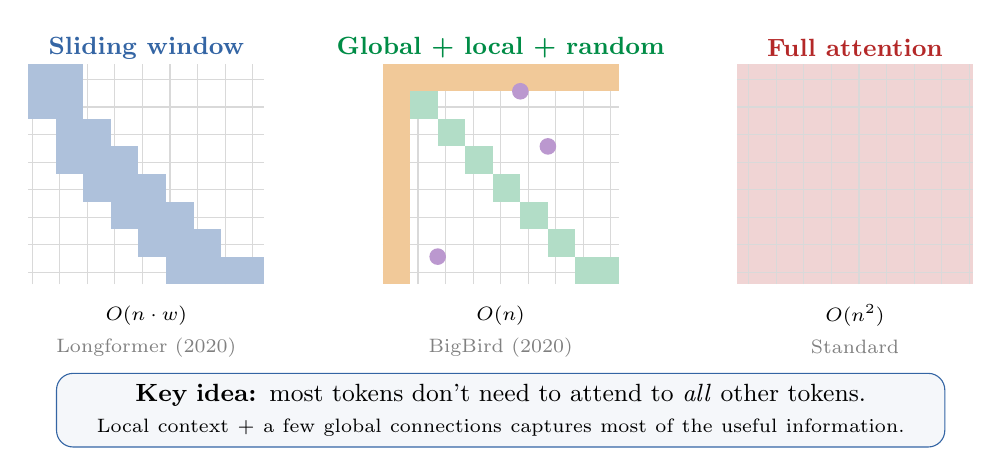
\begin{tikzpicture}
  % Sliding window
  \node[font=\small\bfseries, text=popblue] at (-4.5, 3.2) {Sliding window};
  \fill[white] (-6, 0.2) rectangle (-3, 3);
  \draw[thin, gray!30] (-6, 0.2) grid[step=0.35] (-3, 3);
  % Diagonal band
  \fill[popblue!40] (-6, 2.65) rectangle (-5.65, 3);
  \fill[popblue!40] (-6, 2.3) rectangle (-5.3, 3);
  \fill[popblue!40] (-5.65, 1.95) rectangle (-5.3, 2.65);
  \fill[popblue!40] (-5.65, 1.6) rectangle (-4.95, 2.3);
  \fill[popblue!40] (-5.3, 1.25) rectangle (-4.6, 1.95);
  \fill[popblue!40] (-4.95, 0.9) rectangle (-4.25, 1.6);
  \fill[popblue!40] (-4.6, 0.55) rectangle (-3.9, 1.25);
  \fill[popblue!40] (-4.25, 0.2) rectangle (-3.55, 0.9);
  \fill[popblue!40] (-3.9, 0.2) rectangle (-3, 0.55);
  \node[font=\scriptsize] at (-4.5, -0.2) {$O(n \cdot w)$};
  \node[font=\scriptsize, text=gray] at (-4.5, -0.6) {Longformer (2020)};

  % Global + local + random
  \node[font=\small\bfseries, text=paramgreen] at (0, 3.2) {Global + local + random};
  \fill[white] (-1.5, 0.2) rectangle (1.5, 3);
  \draw[thin, gray!30] (-1.5, 0.2) grid[step=0.35] (1.5, 3);
  % Diagonal band (local)
  \fill[paramgreen!30] (-1.5, 2.65) rectangle (-1.15, 3);
  \fill[paramgreen!30] (-1.15, 2.3) rectangle (-0.8, 2.65);
  \fill[paramgreen!30] (-0.8, 1.95) rectangle (-0.45, 2.3);
  \fill[paramgreen!30] (-0.45, 1.6) rectangle (-0.1, 1.95);
  \fill[paramgreen!30] (-0.1, 1.25) rectangle (0.25, 1.6);
  \fill[paramgreen!30] (0.25, 0.9) rectangle (0.6, 1.25);
  \fill[paramgreen!30] (0.6, 0.55) rectangle (0.95, 0.9);
  \fill[paramgreen!30] (0.95, 0.2) rectangle (1.5, 0.55);
  % Global row/column (first token)
  \fill[orange1!40] (-1.5, 2.65) rectangle (1.5, 3);
  \fill[orange1!40] (-1.5, 0.2) rectangle (-1.15, 3);
  % Random dots
  \fill[violet1!50] (0.25, 2.65) circle (3pt);
  \fill[violet1!50] (-0.8, 0.55) circle (3pt);
  \fill[violet1!50] (0.6, 1.95) circle (3pt);
  \node[font=\scriptsize] at (0, -0.2) {$O(n)$};
  \node[font=\scriptsize, text=gray] at (0, -0.6) {BigBird (2020)};

  % Full attention for comparison
  \node[font=\small\bfseries, text=warnred] at (4.5, 3.2) {Full attention};
  \fill[warnred!20] (3, 0.2) rectangle (6, 3);
  \draw[thin, gray!30] (3, 0.2) grid[step=0.35] (6, 3);
  \node[font=\scriptsize] at (4.5, -0.2) {$O(n^2)$};
  \node[font=\scriptsize, text=gray] at (4.5, -0.6) {Standard};

  % Bottom insight
  \node[draw=popblue, fill=popblue!5, rounded corners=6pt, text width=11cm, align=center, inner sep=4pt, font=\small] at (0, -1.4) {
    \textbf{Key idea:} most tokens don't need to attend to \textit{all} other tokens.\\
    {\scriptsize Local context + a few global connections captures most of the useful information.}
  };
\end{tikzpicture}
\end{center}
\end{frame}

% ============================================================
% LINEAR ATTENTION APPROXIMATIONS
% ============================================================
\begin{frame}
\frametitle{Linear attention approximations}

\begin{center}
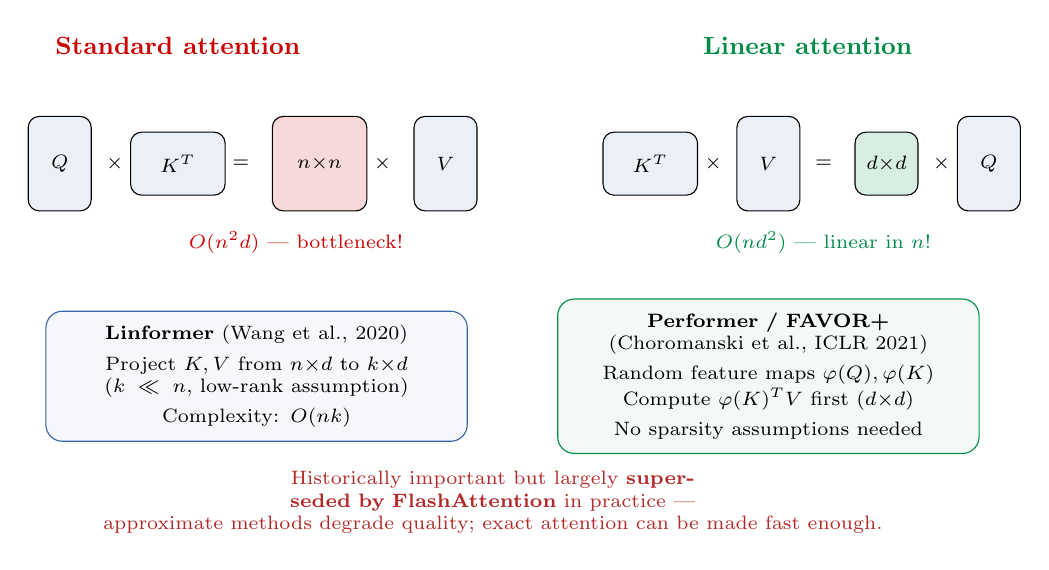
\begin{tikzpicture}
  % Standard attention
  \node[font=\small\bfseries, text=sampred] at (-4, 3) {Standard attention};
  \node[draw, rounded corners=4pt, fill=popblue!10, font=\scriptsize, minimum width=0.8cm, minimum height=1.2cm] (Q1) at (-5.5, 1.5) {$Q$};
  \node[font=\scriptsize] at (-4.8, 1.5) {$\times$};
  \node[draw, rounded corners=4pt, fill=popblue!10, font=\scriptsize, minimum width=1.2cm, minimum height=0.8cm] (K1) at (-4, 1.5) {$K^T$};
  \node[font=\scriptsize] at (-3.2, 1.5) {$=$};
  \node[draw, rounded corners=4pt, fill=sampred!15, font=\scriptsize, minimum width=1.2cm, minimum height=1.2cm] (A1) at (-2.2, 1.5) {$n{\times}n$};
  \node[font=\scriptsize] at (-1.4, 1.5) {$\times$};
  \node[draw, rounded corners=4pt, fill=popblue!10, font=\scriptsize, minimum width=0.8cm, minimum height=1.2cm] (V1) at (-0.6, 1.5) {$V$};
  \node[font=\scriptsize, text=sampred] at (-2.5, 0.5) {$O(n^2 d)$ --- bottleneck!};

  % Linear attention
  \node[font=\small\bfseries, text=paramgreen] at (4, 3) {Linear attention};
  \node[draw, rounded corners=4pt, fill=popblue!10, font=\scriptsize, minimum width=1.2cm, minimum height=0.8cm] (K2) at (2, 1.5) {$K^T$};
  \node[font=\scriptsize] at (2.8, 1.5) {$\times$};
  \node[draw, rounded corners=4pt, fill=popblue!10, font=\scriptsize, minimum width=0.8cm, minimum height=1.2cm] (V2) at (3.5, 1.5) {$V$};
  \node[font=\scriptsize] at (4.2, 1.5) {$=$};
  \node[draw, rounded corners=4pt, fill=paramgreen!15, font=\scriptsize, minimum width=0.8cm, minimum height=0.8cm] (B2) at (5, 1.5) {$d{\times}d$};
  \node[font=\scriptsize] at (5.7, 1.5) {$\times$};
  \node[draw, rounded corners=4pt, fill=popblue!10, font=\scriptsize, minimum width=0.8cm, minimum height=1.2cm] (Q2) at (6.3, 1.5) {$Q$};
  \node[font=\scriptsize, text=paramgreen] at (4.2, 0.5) {$O(n d^2)$ --- linear in $n$!};

  % Methods
  \node[draw=popblue, fill=popblue!5, rounded corners=6pt, text width=5cm, align=center, inner sep=5pt, font=\scriptsize] at (-3, -1.2) {
    \textbf{Linformer} (Wang et al., 2020)\\[3pt]
    Project $K, V$ from $n{\times}d$ to $k{\times}d$\\
    ($k \ll n$, low-rank assumption)\\[3pt]
    Complexity: $O(nk)$
  };

  \node[draw=paramgreen, fill=paramgreen!5, rounded corners=6pt, text width=5cm, align=center, inner sep=5pt, font=\scriptsize] at (3.5, -1.2) {
    \textbf{Performer / FAVOR+}\\(Choromanski et al., ICLR 2021)\\[3pt]
    Random feature maps $\varphi(Q), \varphi(K)$\\
    Compute $\varphi(K)^T V$ first ($d{\times}d$)\\[3pt]
    No sparsity assumptions needed
  };

  % Caveat
  \node[font=\scriptsize, text=warnred, text width=10cm, align=center] at (0, -2.8) {
    Historically important but largely \textbf{superseded by FlashAttention} in practice ---\\
    approximate methods degrade quality; exact attention can be made fast enough.
  };
\end{tikzpicture}
\end{center}
\end{frame}

% ============================================================
% FLASH ATTENTION
% ============================================================
\begin{frame}
\frametitle{FlashAttention: the IO-aware revolution}

\begin{center}
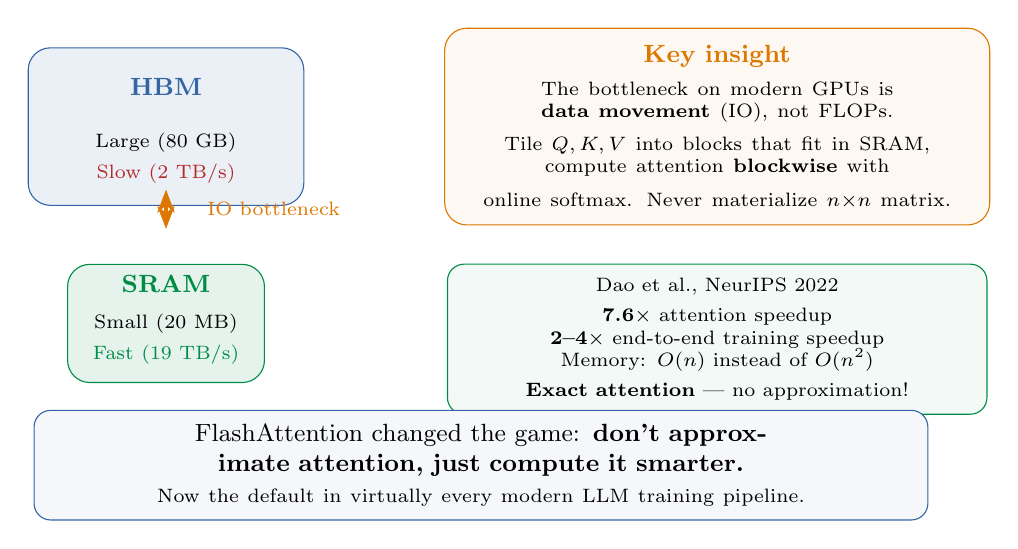
\begin{tikzpicture}
  % GPU memory hierarchy
  \node[draw=popblue, fill=popblue!10, rounded corners=8pt, minimum width=3.5cm, minimum height=2cm, font=\small] (hbm) at (-4, 2) {};
  \node[font=\small\bfseries, text=popblue] at (-4, 2.5) {HBM};
  \node[font=\scriptsize] at (-4, 1.8) {Large (80 GB)};
  \node[font=\scriptsize, text=warnred] at (-4, 1.4) {Slow (2 TB/s)};

  \node[draw=paramgreen, fill=paramgreen!10, rounded corners=8pt, minimum width=2.5cm, minimum height=1.5cm, font=\small] (sram) at (-4, -0.5) {};
  \node[font=\small\bfseries, text=paramgreen] at (-4, 0) {SRAM};
  \node[font=\scriptsize] at (-4, -0.5) {Small (20 MB)};
  \node[font=\scriptsize, text=paramgreen] at (-4, -0.9) {Fast (19 TB/s)};

  \draw[Stealth-Stealth, very thick, orange1] (-4, 0.7) -- (-4, 1.2);
  \node[font=\scriptsize, text=orange1, right] at (-3.6, 0.95) {IO bottleneck};

  % FlashAttention idea
  \node[draw=orange1, fill=orange1!5, rounded corners=8pt, text width=6.5cm, align=center, inner sep=6pt] at (3, 2) {
    {\small\bfseries\textcolor{orange1}{Key insight}}\\[4pt]
    {\scriptsize The bottleneck on modern GPUs is\\
    \textbf{data movement} (IO), not FLOPs.\\[4pt]
    Tile $Q, K, V$ into blocks that fit in SRAM,\\
    compute attention \textbf{blockwise} with\\
    online softmax. Never materialize $n{\times}n$ matrix.}
  };

  % Results
  \node[draw=paramgreen, fill=paramgreen!5, rounded corners=6pt, text width=6.5cm, align=center, inner sep=5pt, font=\scriptsize] at (3, -0.7) {
    Dao et al., NeurIPS 2022\\[3pt]
    \textbf{7.6$\times$} attention speedup\\
    \textbf{2--4$\times$} end-to-end training speedup\\
    Memory: $O(n)$ instead of $O(n^2)$\\[3pt]
    \textbf{Exact attention} --- no approximation!
  };

  % Bottom
  \node[draw=popblue, fill=popblue!5, rounded corners=6pt, text width=11cm, align=center, inner sep=5pt, font=\small] at (0, -2.3) {
    FlashAttention changed the game: \textbf{don't approximate attention, just compute it smarter.}\\
    {\scriptsize Now the default in virtually every modern LLM training pipeline.}
  };
\end{tikzpicture}
\end{center}
\end{frame}

% ============================================================
% FLASH ATTENTION 2 & 3
% ============================================================
\begin{frame}
\frametitle{FlashAttention evolution}
\vspace{-0.2cm}
\begin{center}
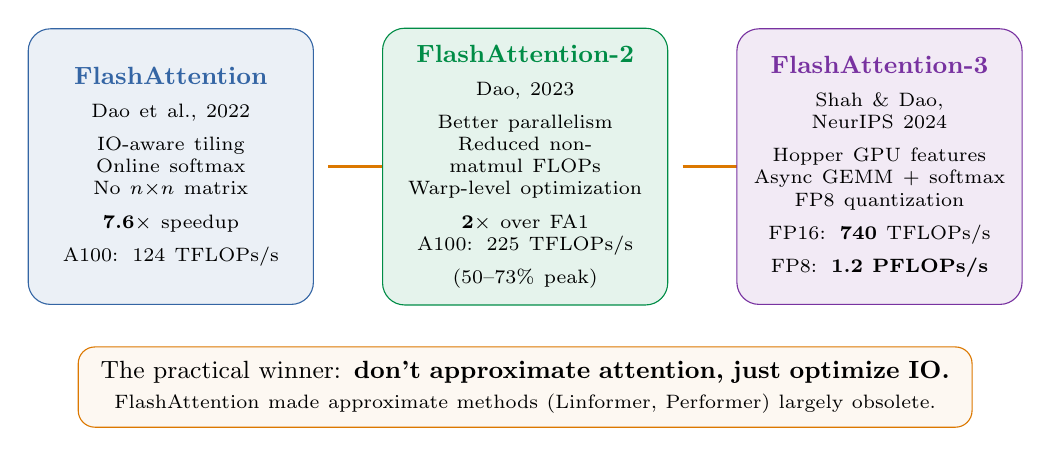
\begin{tikzpicture}
  % FA1
  \node[draw=popblue, fill=popblue!10, rounded corners=8pt, text width=3.2cm, align=center, inner sep=6pt, minimum height=3.5cm] at (-4.5, 1) {
    {\small\bfseries\textcolor{popblue}{FlashAttention}}\\[4pt]
    {\scriptsize Dao et al., 2022\\[4pt]
    IO-aware tiling\\
    Online softmax\\
    No $n{\times}n$ matrix\\[4pt]
    \textbf{7.6$\times$} speedup\\
    A100: 124 TFLOPs/s}
  };

  % Arrow
  \draw[-Stealth, very thick, orange1] (-2.5, 1) -- (-1.5, 1);

  % FA2
  \node[draw=paramgreen, fill=paramgreen!10, rounded corners=8pt, text width=3.2cm, align=center, inner sep=6pt, minimum height=3.5cm] at (0, 1) {
    {\small\bfseries\textcolor{paramgreen}{FlashAttention-2}}\\[4pt]
    {\scriptsize Dao, 2023\\[4pt]
    Better parallelism\\
    Reduced non-matmul FLOPs\\
    Warp-level optimization\\[4pt]
    \textbf{2$\times$} over FA1\\
    A100: 225 TFLOPs/s\\
    (50--73\% peak)}
  };

  % Arrow
  \draw[-Stealth, very thick, orange1] (2, 1) -- (3, 1);

  % FA3
  \node[draw=violet1, fill=violet1!10, rounded corners=8pt, text width=3.2cm, align=center, inner sep=6pt, minimum height=3.5cm] at (4.5, 1) {
    {\small\bfseries\textcolor{violet1}{FlashAttention-3}}\\[4pt]
    {\scriptsize Shah \& Dao, NeurIPS 2024\\[4pt]
    Hopper GPU features\\
    Async GEMM + softmax\\
    FP8 quantization\\[4pt]
    FP16: \textbf{740} TFLOPs/s\\
    FP8: \textbf{1.2 PFLOPs/s}}
  };

  % Bottom
  \node[draw=orange1, fill=orange1!5, rounded corners=6pt, text width=11cm, align=center, inner sep=5pt, font=\small] at (0, -1.8) {
    The practical winner: \textbf{don't approximate attention, just optimize IO.}\\
    {\scriptsize FlashAttention made approximate methods (Linformer, Performer) largely obsolete.}
  };
\end{tikzpicture}
\end{center}
\end{frame}

% ============================================================
% MQA / GQA
% ============================================================
\begin{frame}
\frametitle{Multi-Query \& Grouped-Query Attention}

\begin{center}
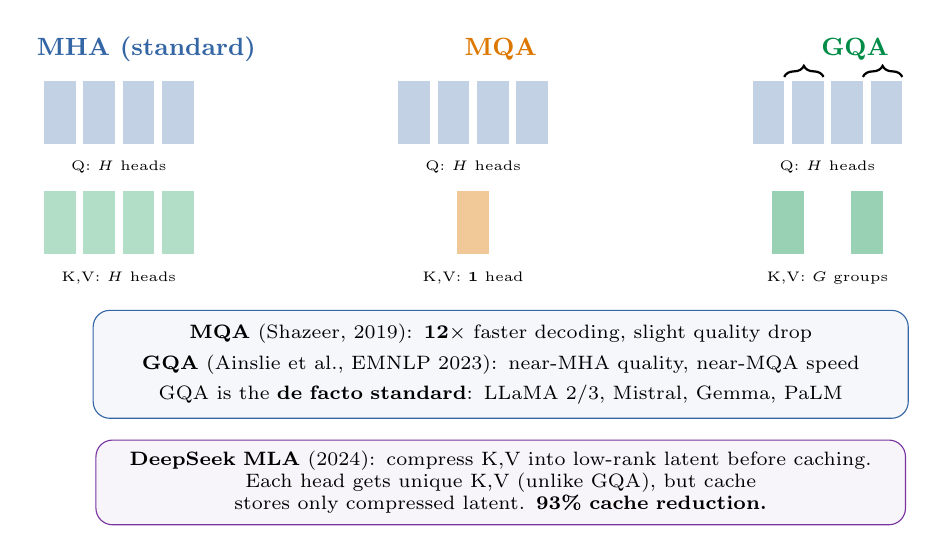
\begin{tikzpicture}
  % MHA
  \node[font=\small\bfseries, text=popblue] at (-4.5, 3.2) {MHA (standard)};
  % Q heads
  \fill[popblue!30] (-5.8, 2) rectangle (-5.4, 2.8);
  \fill[popblue!30] (-5.3, 2) rectangle (-4.9, 2.8);
  \fill[popblue!30] (-4.8, 2) rectangle (-4.4, 2.8);
  \fill[popblue!30] (-4.3, 2) rectangle (-3.9, 2.8);
  \node[font=\tiny] at (-4.85, 1.7) {Q: $H$ heads};
  % K heads
  \fill[paramgreen!30] (-5.8, 0.6) rectangle (-5.4, 1.4);
  \fill[paramgreen!30] (-5.3, 0.6) rectangle (-4.9, 1.4);
  \fill[paramgreen!30] (-4.8, 0.6) rectangle (-4.4, 1.4);
  \fill[paramgreen!30] (-4.3, 0.6) rectangle (-3.9, 1.4);
  \node[font=\tiny] at (-4.85, 0.3) {K,V: $H$ heads};

  % MQA
  \node[font=\small\bfseries, text=orange1] at (0, 3.2) {MQA};
  % Q heads
  \fill[popblue!30] (-1.3, 2) rectangle (-0.9, 2.8);
  \fill[popblue!30] (-0.8, 2) rectangle (-0.4, 2.8);
  \fill[popblue!30] (-0.3, 2) rectangle (0.1, 2.8);
  \fill[popblue!30] (0.2, 2) rectangle (0.6, 2.8);
  \node[font=\tiny] at (-0.35, 1.7) {Q: $H$ heads};
  % K head (single)
  \fill[orange1!40] (-0.55, 0.6) rectangle (-0.15, 1.4);
  \node[font=\tiny] at (-0.35, 0.3) {K,V: \textbf{1} head};

  % GQA
  \node[font=\small\bfseries, text=paramgreen] at (4.5, 3.2) {GQA};
  % Q heads
  \fill[popblue!30] (3.2, 2) rectangle (3.6, 2.8);
  \fill[popblue!30] (3.7, 2) rectangle (4.1, 2.8);
  \fill[popblue!30] (4.2, 2) rectangle (4.6, 2.8);
  \fill[popblue!30] (4.7, 2) rectangle (5.1, 2.8);
  \node[font=\tiny] at (4.15, 1.7) {Q: $H$ heads};
  % K groups
  \fill[paramgreen!40] (3.45, 0.6) rectangle (3.85, 1.4);
  \fill[paramgreen!40] (4.45, 0.6) rectangle (4.85, 1.4);
  \node[font=\tiny] at (4.15, 0.3) {K,V: $G$ groups};

  % Brackets showing grouping
  \draw[thick, decorate, decoration={brace, amplitude=4pt}] (3.6, 2.85) -- (4.1, 2.85);
  \draw[thick, decorate, decoration={brace, amplitude=4pt}] (4.6, 2.85) -- (5.1, 2.85);

  % Comparison
  \node[draw=popblue, fill=popblue!5, rounded corners=6pt, text width=10cm, align=center, inner sep=5pt, font=\scriptsize] at (0, -0.8) {
    \textbf{MQA} (Shazeer, 2019): \textbf{12$\times$} faster decoding, slight quality drop\\[3pt]
    \textbf{GQA} (Ainslie et al., EMNLP 2023): near-MHA quality, near-MQA speed\\[3pt]
    GQA is the \textbf{de facto standard}: LLaMA 2/3, Mistral, Gemma, PaLM
  };

  % DeepSeek MLA
  \node[draw=violet1, fill=violet1!5, rounded corners=6pt, text width=10cm, align=center, inner sep=4pt, font=\scriptsize] at (0, -2.3) {
    \textbf{DeepSeek MLA} (2024): compress K,V into low-rank latent before caching.\\
    Each head gets unique K,V (unlike GQA), but cache stores only compressed latent. \textbf{93\% cache reduction.}
  };
\end{tikzpicture}
\end{center}
\end{frame}

% ============================================================
% KV CACHE: THE INFERENCE BOTTLENECK
% ============================================================
\begin{frame}
\frametitle{KV cache: the inference bottleneck}

\begin{center}
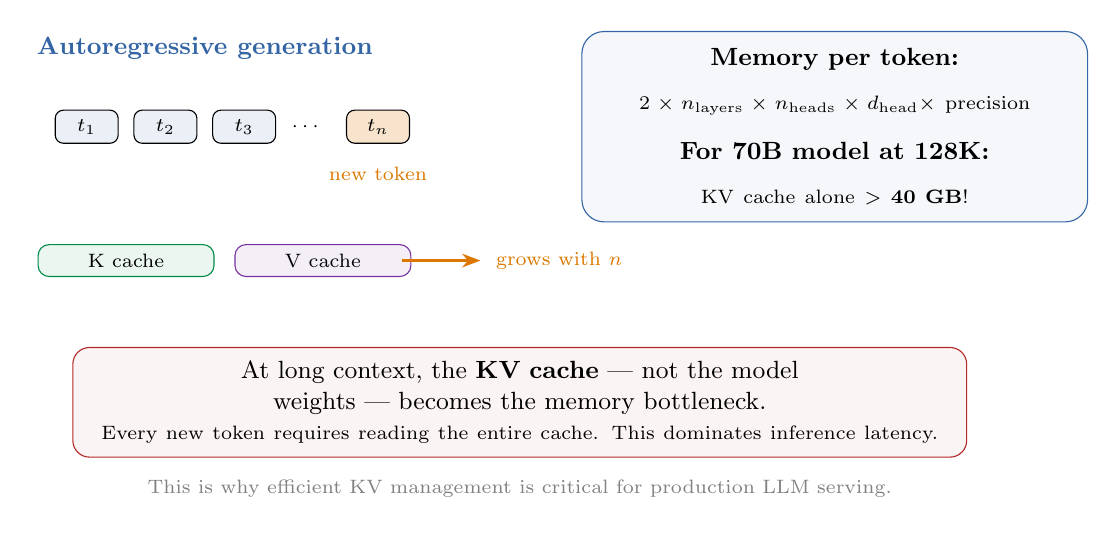
\begin{tikzpicture}
  % Autoregressive generation
  \node[font=\small\bfseries, text=popblue] at (-4, 3) {Autoregressive generation};

  % Existing tokens
  \node[draw, rounded corners=3pt, fill=popblue!10, font=\scriptsize, minimum width=0.8cm] at (-5.5, 2) {$t_1$};
  \node[draw, rounded corners=3pt, fill=popblue!10, font=\scriptsize, minimum width=0.8cm] at (-4.5, 2) {$t_2$};
  \node[draw, rounded corners=3pt, fill=popblue!10, font=\scriptsize, minimum width=0.8cm] at (-3.5, 2) {$t_3$};
  \node[font=\scriptsize] at (-2.7, 2) {$\cdots$};
  \node[draw, rounded corners=3pt, fill=orange1!20, font=\scriptsize\bfseries, minimum width=0.8cm] at (-1.8, 2) {$t_n$};
  \node[font=\scriptsize, text=orange1] at (-1.8, 1.4) {new token};

  % KV cache growing
  \node[draw=paramgreen, fill=paramgreen!8, rounded corners=4pt, font=\scriptsize, text width=2cm, align=center] at (-5, 0.3) {K cache};
  \node[draw=violet1, fill=violet1!8, rounded corners=4pt, font=\scriptsize, text width=2cm, align=center] at (-2.5, 0.3) {V cache};
  \draw[-Stealth, thick, orange1] (-1.5, 0.3) -- (-0.5, 0.3);
  \node[font=\scriptsize, text=orange1] at (0.5, 0.3) {grows with $n$};

  % Memory formula
  \node[draw=popblue, fill=popblue!5, rounded corners=8pt, text width=6cm, align=center, inner sep=6pt] at (4, 2) {
    {\small\bfseries Memory per token:}\\[4pt]
    {\scriptsize $2 \times n_{\text{layers}} \times n_{\text{heads}} \times d_{\text{head}} \times$ precision}\\[6pt]
    {\small\bfseries For 70B model at 128K:}\\[4pt]
    {\scriptsize KV cache alone $>$ \textbf{40 GB}!}
  };

  % Bottom insight
  \node[draw=warnred, fill=warnred!5, rounded corners=6pt, text width=11cm, align=center, inner sep=5pt, font=\small] at (0, -1.5) {
    At long context, the \textbf{KV cache} --- not the model weights --- becomes the memory bottleneck.\\
    {\scriptsize Every new token requires reading the entire cache. This dominates inference latency.}
  };

  \node[font=\scriptsize, text=gray] at (0, -2.6) {This is why efficient KV management is critical for production LLM serving.};
\end{tikzpicture}
\end{center}
\end{frame}

% ============================================================
% KV CACHE OPTIMIZATION
% ============================================================
\begin{frame}
\frametitle{KV cache optimization}

\begin{center}
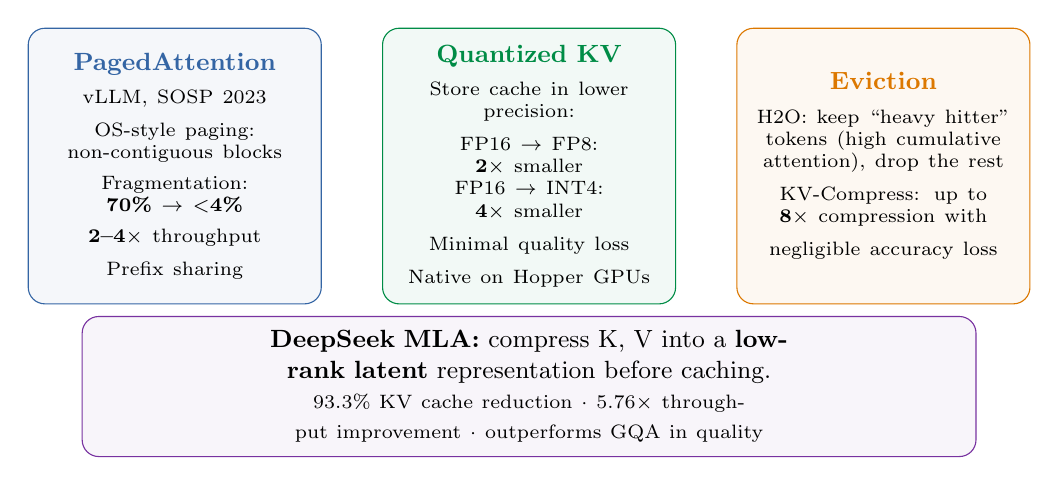
\begin{tikzpicture}
  % PagedAttention
  \node[draw=popblue, fill=popblue!5, rounded corners=6pt, text width=3.3cm, align=center, inner sep=6pt, minimum height=3.5cm] at (-4.5, 1) {
    {\small\bfseries\textcolor{popblue}{PagedAttention}}\\[4pt]
    {\scriptsize vLLM, SOSP 2023\\[4pt]
    OS-style paging:\\
    non-contiguous blocks\\[3pt]
    Fragmentation:\\
    \textbf{70\%} $\to$ \textbf{$<$4\%}\\[3pt]
    \textbf{2--4$\times$} throughput\\
    Prefix sharing}
  };

  % Quantized KV
  \node[draw=paramgreen, fill=paramgreen!5, rounded corners=6pt, text width=3.3cm, align=center, inner sep=6pt, minimum height=3.5cm] at (0, 1) {
    {\small\bfseries\textcolor{paramgreen}{Quantized KV}}\\[4pt]
    {\scriptsize Store cache in lower\\precision:\\[4pt]
    FP16 $\to$ FP8: \textbf{2$\times$} smaller\\
    FP16 $\to$ INT4: \textbf{4$\times$} smaller\\[4pt]
    Minimal quality loss\\
    Native on Hopper GPUs}
  };

  % Eviction
  \node[draw=orange1, fill=orange1!5, rounded corners=6pt, text width=3.3cm, align=center, inner sep=6pt, minimum height=3.5cm] at (4.5, 1) {
    {\small\bfseries\textcolor{orange1}{Eviction}}\\[4pt]
    {\scriptsize H2O: keep ``heavy hitter''\\tokens (high cumulative\\attention), drop the rest\\[4pt]
    KV-Compress: up to\\
    \textbf{8$\times$} compression with\\
    negligible accuracy loss}
  };

  % DeepSeek MLA
  \node[draw=violet1, fill=violet1!5, rounded corners=6pt, text width=11cm, align=center, inner sep=5pt, font=\small] at (0, -1.8) {
    \textbf{DeepSeek MLA:} compress K, V into a \textbf{low-rank latent} representation before caching.\\
    {\scriptsize 93.3\% KV cache reduction $\cdot$ 5.76$\times$ throughput improvement $\cdot$ outperforms GQA in quality}
  };
\end{tikzpicture}
\end{center}
\end{frame}

% ============================================================
% POSITIONAL ENCODING FOR LENGTH
% ============================================================
\begin{frame}
\frametitle{Positional encoding for length}

\begin{center}
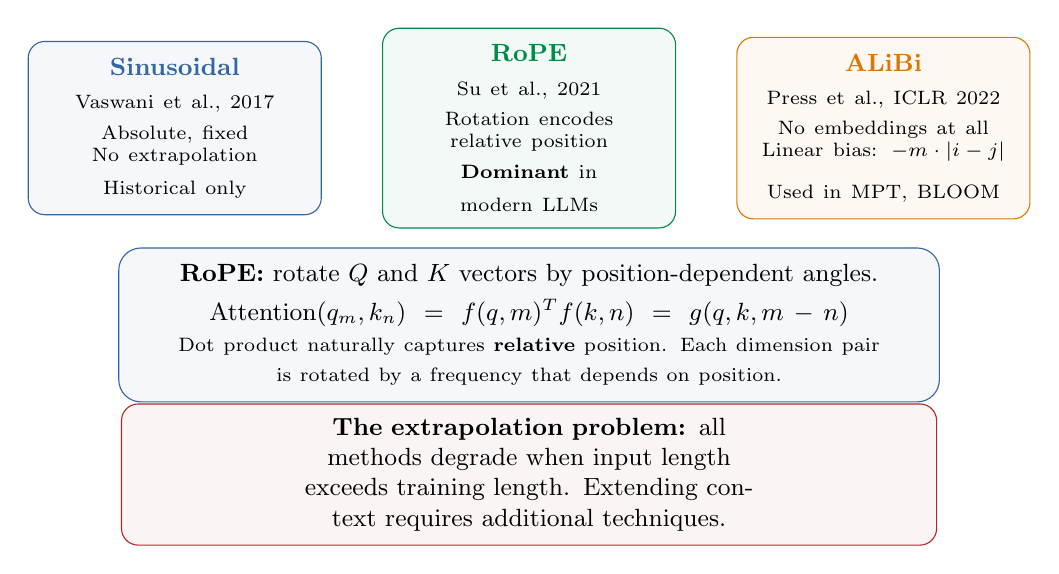
\begin{tikzpicture}
  % Sinusoidal
  \node[draw=popblue, fill=popblue!5, rounded corners=6pt, text width=3.3cm, align=center, inner sep=6pt] at (-4.5, 2.2) {
    {\small\bfseries\textcolor{popblue}{Sinusoidal}}\\[4pt]
    {\scriptsize Vaswani et al., 2017\\[3pt]
    Absolute, fixed\\
    No extrapolation\\
    Historical only}
  };

  % RoPE
  \node[draw=paramgreen, fill=paramgreen!5, rounded corners=6pt, text width=3.3cm, align=center, inner sep=6pt] at (0, 2.2) {
    {\small\bfseries\textcolor{paramgreen}{RoPE}}\\[4pt]
    {\scriptsize Su et al., 2021\\[3pt]
    Rotation encodes\\relative position\\[3pt]
    \textbf{Dominant} in\\modern LLMs}
  };

  % ALiBi
  \node[draw=orange1, fill=orange1!5, rounded corners=6pt, text width=3.3cm, align=center, inner sep=6pt] at (4.5, 2.2) {
    {\small\bfseries\textcolor{orange1}{ALiBi}}\\[4pt]
    {\scriptsize Press et al., ICLR 2022\\[3pt]
    No embeddings at all\\
    Linear bias: $-m \cdot |i-j|$\\[3pt]
    Used in MPT, BLOOM}
  };

  % RoPE detail
  \node[draw=popblue, fill=popblue!5, rounded corners=8pt, text width=10cm, align=center, inner sep=6pt, font=\small] at (0, -0.3) {
    \textbf{RoPE:} rotate $Q$ and $K$ vectors by position-dependent angles.\\[3pt]
    $\text{Attention}(q_m, k_n) = f(q, m)^T f(k, n) = g(q, k, m-n)$\\[3pt]
    {\scriptsize Dot product naturally captures \textbf{relative} position. Each dimension pair\\
    is rotated by a frequency that depends on position.}
  };

  % Problem
  \node[draw=warnred, fill=warnred!5, rounded corners=6pt, text width=10cm, align=center, inner sep=5pt, font=\small] at (0, -2.2) {
    \textbf{The extrapolation problem:} all methods degrade when input length\\
    exceeds training length. Extending context requires additional techniques.
  };
\end{tikzpicture}
\end{center}
\end{frame}

% ============================================================
% CONTEXT WINDOW EXTENSION
% ============================================================
\begin{frame}
\frametitle{Context window extension}
\vspace{-0.2cm}
\begin{center}
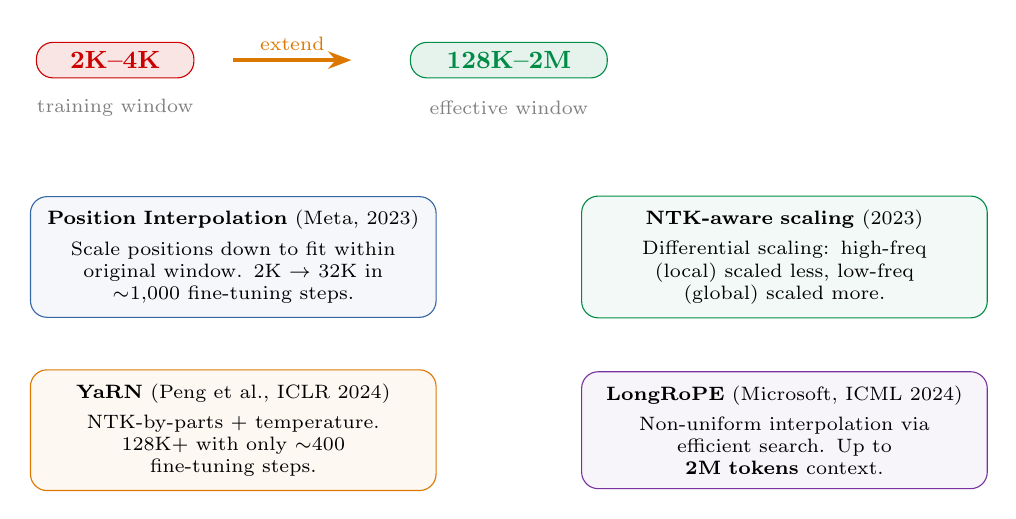
\begin{tikzpicture}
  % Training window
  \node[draw=sampred, fill=sampred!10, rounded corners=6pt, font=\small\bfseries, minimum width=2cm, text=sampred] (train) at (-5, 2.5) {2K--4K};
  \node[font=\scriptsize, text=gray] at (-5, 1.9) {training window};

  % Arrow
  \draw[-Stealth, very thick, orange1] (-3.5, 2.5) -- (-2, 2.5);
  \node[font=\scriptsize, text=orange1, above] at (-2.75, 2.5) {extend};

  % Extended window
  \node[draw=paramgreen, fill=paramgreen!10, rounded corners=6pt, font=\small\bfseries, minimum width=2.5cm, text=paramgreen] (ext) at (0, 2.5) {128K--2M};
  \node[font=\scriptsize, text=gray] at (0, 1.9) {effective window};

  % Methods
  \node[draw=popblue, fill=popblue!5, rounded corners=6pt, text width=4.8cm, align=center, inner sep=5pt, font=\scriptsize] at (-3.5, 0) {
    \textbf{Position Interpolation} (Meta, 2023)\\[3pt]
    Scale positions down to fit within\\
    original window. 2K $\to$ 32K in\\
    $\sim$1,000 fine-tuning steps.
  };

  \node[draw=paramgreen, fill=paramgreen!5, rounded corners=6pt, text width=4.8cm, align=center, inner sep=5pt, font=\scriptsize] at (3.5, 0) {
    \textbf{NTK-aware scaling} (2023)\\[3pt]
    Differential scaling: high-freq\\
    (local) scaled less, low-freq\\
    (global) scaled more.
  };

  \node[draw=orange1, fill=orange1!5, rounded corners=6pt, text width=4.8cm, align=center, inner sep=5pt, font=\scriptsize] at (-3.5, -2.2) {
    \textbf{YaRN} (Peng et al., ICLR 2024)\\[3pt]
    NTK-by-parts + temperature.\\
    128K+ with only $\sim$400\\
    fine-tuning steps.
  };

  \node[draw=violet1, fill=violet1!5, rounded corners=6pt, text width=4.8cm, align=center, inner sep=5pt, font=\scriptsize] at (3.5, -2.2) {
    \textbf{LongRoPE} (Microsoft, ICML 2024)\\[3pt]
    Non-uniform interpolation via\\
    efficient search. Up to\\
    \textbf{2M tokens} context.
  };
\end{tikzpicture}
\end{center}
\end{frame}

% ============================================================
% RING ATTENTION
% ============================================================
\begin{frame}
\frametitle{Ring Attention}

\begin{center}
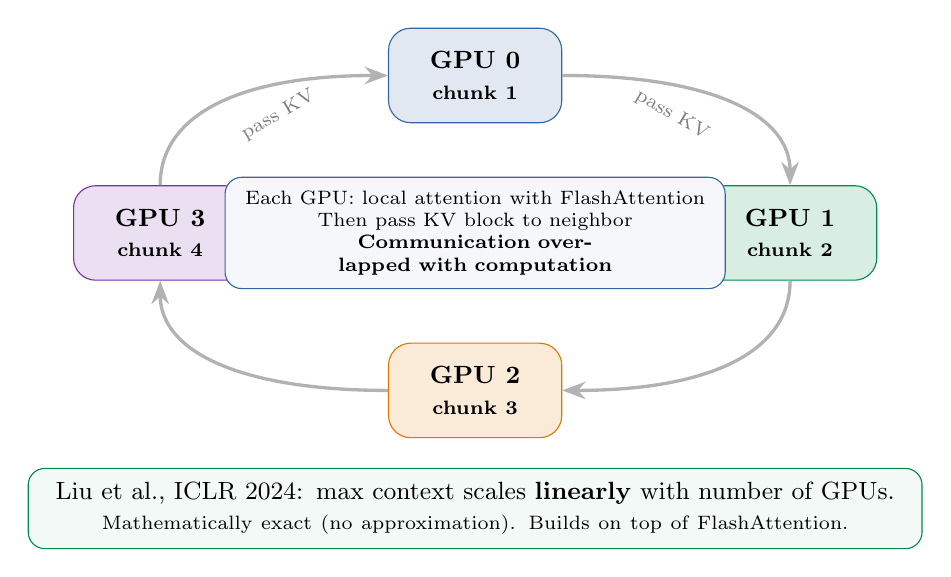
\begin{tikzpicture}
  % Ring of 4 GPUs
  \node[draw=popblue, fill=popblue!15, rounded corners=8pt, minimum width=2.2cm, minimum height=1.2cm, font=\small\bfseries, align=center] (g0) at (0, 2.5) {GPU 0\\{\scriptsize chunk 1}};
  \node[draw=paramgreen, fill=paramgreen!15, rounded corners=8pt, minimum width=2.2cm, minimum height=1.2cm, font=\small\bfseries, align=center] (g1) at (4, 0.5) {GPU 1\\{\scriptsize chunk 2}};
  \node[draw=orange1, fill=orange1!15, rounded corners=8pt, minimum width=2.2cm, minimum height=1.2cm, font=\small\bfseries, align=center] (g2) at (0, -1.5) {GPU 2\\{\scriptsize chunk 3}};
  \node[draw=violet1, fill=violet1!15, rounded corners=8pt, minimum width=2.2cm, minimum height=1.2cm, font=\small\bfseries, align=center] (g3) at (-4, 0.5) {GPU 3\\{\scriptsize chunk 4}};

  % Ring arrows (clockwise)
  \draw[-Stealth, very thick, gray!60] (g0.east) .. controls (3, 2.5) and (4, 2) .. (g1.north);
  \draw[-Stealth, very thick, gray!60] (g1.south) .. controls (4, -1) and (3, -1.5) .. (g2.east);
  \draw[-Stealth, very thick, gray!60] (g2.west) .. controls (-3, -1.5) and (-4, -1) .. (g3.south);
  \draw[-Stealth, very thick, gray!60] (g3.north) .. controls (-4, 2) and (-3, 2.5) .. (g0.west);

  \node[font=\scriptsize, text=gray, rotate=-30] at (2.5, 2) {pass KV};
  \node[font=\scriptsize, text=gray, rotate=30] at (-2.5, 2) {pass KV};

  % Key properties
  \node[draw=popblue, fill=popblue!5, rounded corners=6pt, text width=6cm, align=center, inner sep=5pt, font=\scriptsize] at (0, 0.5) {
    Each GPU: local attention with FlashAttention\\
    Then pass KV block to neighbor\\
    \textbf{Communication overlapped with computation}
  };

  % Bottom
  \node[draw=paramgreen, fill=paramgreen!5, rounded corners=6pt, text width=11cm, align=center, inner sep=5pt, font=\small] at (0, -3) {
    Liu et al., ICLR 2024: max context scales \textbf{linearly} with number of GPUs.\\
    {\scriptsize Mathematically exact (no approximation). Builds on top of FlashAttention.}
  };
\end{tikzpicture}
\end{center}
\end{frame}

% ============================================================
% STATE SPACE MODELS: S4
% ============================================================
\begin{frame}
\frametitle{State Space Models: S4}

\begin{center}
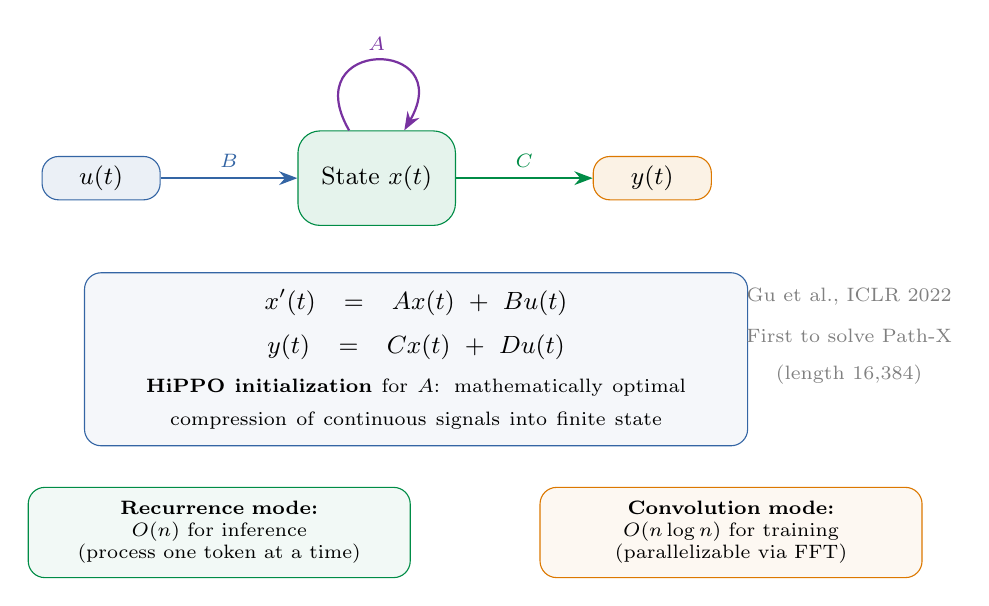
\begin{tikzpicture}
  % SSM diagram
  \node[draw=popblue, fill=popblue!10, rounded corners=6pt, font=\small, minimum width=1.5cm] (input) at (-5, 2) {$u(t)$};
  \node[draw=paramgreen, fill=paramgreen!10, rounded corners=8pt, font=\small, minimum width=2cm, minimum height=1.2cm] (state) at (-1.5, 2) {State $x(t)$};
  \node[draw=orange1, fill=orange1!10, rounded corners=6pt, font=\small, minimum width=1.5cm] (output) at (2, 2) {$y(t)$};

  \draw[-Stealth, thick, popblue] (input) -- node[above, font=\scriptsize] {$B$} (state);
  \draw[-Stealth, thick, paramgreen] (state) -- node[above, font=\scriptsize] {$C$} (output);
  \draw[-Stealth, thick, violet1] (state) to[loop above, looseness=5, out=120, in=60] node[above, font=\scriptsize] {$A$} (state);

  % Equations
  \node[draw=popblue, fill=popblue!5, rounded corners=6pt, text width=8cm, align=center, inner sep=6pt] at (-1, -0.3) {
    {\small $x'(t) = Ax(t) + Bu(t)$}\\[4pt]
    {\small $y(t) = Cx(t) + Du(t)$}\\[6pt]
    {\scriptsize \textbf{HiPPO initialization} for $A$: mathematically optimal\\
    compression of continuous signals into finite state}
  };

  % Dual mode
  \node[draw=paramgreen, fill=paramgreen!5, rounded corners=6pt, text width=4.5cm, align=center, inner sep=5pt, font=\scriptsize] at (-3.5, -2.5) {
    \textbf{Recurrence mode:}\\
    $O(n)$ for inference\\
    (process one token at a time)
  };

  \node[draw=orange1, fill=orange1!5, rounded corners=6pt, text width=4.5cm, align=center, inner sep=5pt, font=\scriptsize] at (3, -2.5) {
    \textbf{Convolution mode:}\\
    $O(n \log n)$ for training\\
    (parallelizable via FFT)
  };

  % Citation
  \node[font=\scriptsize, text=gray] at (4.5, 0.5) {Gu et al., ICLR 2022};
  \node[font=\scriptsize, text=gray] at (4.5, 0) {First to solve Path-X};
  \node[font=\scriptsize, text=gray] at (4.5, -0.5) {(length 16,384)};
\end{tikzpicture}
\end{center}
\end{frame}

% ============================================================
% MAMBA: SELECTIVE STATE SPACES
% ============================================================
\begin{frame}
\frametitle{Mamba: selective state spaces}

\begin{center}
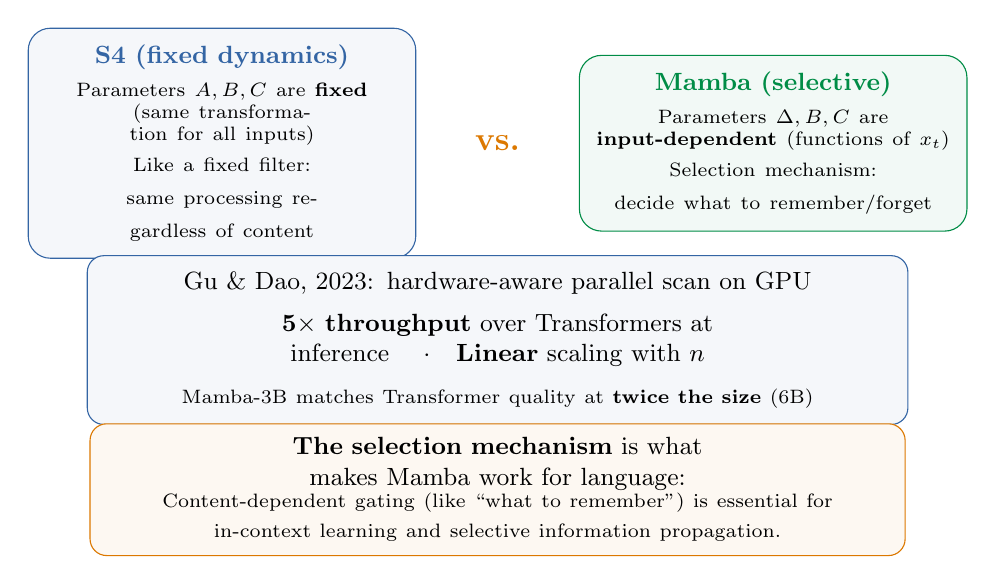
\begin{tikzpicture}
  % S4 (fixed)
  \node[draw=popblue, fill=popblue!5, rounded corners=8pt, text width=4.5cm, align=center, inner sep=6pt] at (-3.5, 2.2) {
    {\small\bfseries\textcolor{popblue}{S4 (fixed dynamics)}}\\[4pt]
    {\scriptsize Parameters $A, B, C$ are \textbf{fixed}\\
    (same transformation for all inputs)\\[3pt]
    Like a fixed filter:\\
    same processing regardless of content}
  };

  % vs
  \node[font=\large\bfseries, text=orange1] at (0, 2.2) {vs.};

  % Mamba (selective)
  \node[draw=paramgreen, fill=paramgreen!5, rounded corners=8pt, text width=4.5cm, align=center, inner sep=6pt] at (3.5, 2.2) {
    {\small\bfseries\textcolor{paramgreen}{Mamba (selective)}}\\[4pt]
    {\scriptsize Parameters $\Delta, B, C$ are\\
    \textbf{input-dependent} (functions of $x_t$)\\[3pt]
    Selection mechanism:\\
    decide what to remember/forget}
  };

  % Key results
  \node[draw=popblue, fill=popblue!5, rounded corners=6pt, text width=10cm, align=center, inner sep=6pt, font=\small] at (0, -0.3) {
    Gu \& Dao, 2023: hardware-aware parallel scan on GPU\\[4pt]
    \textbf{5$\times$ throughput} over Transformers at inference \quad$\cdot$\quad \textbf{Linear} scaling with $n$\\[4pt]
    {\scriptsize Mamba-3B matches Transformer quality at \textbf{twice the size} (6B)}
  };

  % Bottom
  \node[draw=orange1, fill=orange1!5, rounded corners=6pt, text width=10cm, align=center, inner sep=5pt, font=\small] at (0, -2.2) {
    \textbf{The selection mechanism} is what makes Mamba work for language:\\
    {\scriptsize Content-dependent gating (like ``what to remember'') is essential for\\
    in-context learning and selective information propagation.}
  };
\end{tikzpicture}
\end{center}
\end{frame}

% ============================================================
% MAMBA-2 & HYBRIDS
% ============================================================
\begin{frame}
\frametitle{Mamba-2 \& hybrid architectures}
\vspace{-0.2cm}
\begin{center}
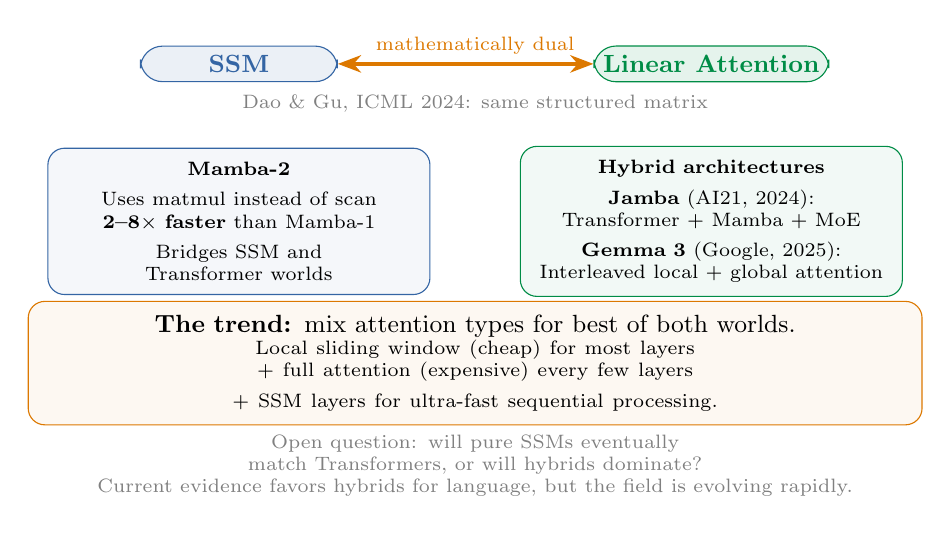
\begin{tikzpicture}
  % Duality
  \node[draw=popblue, fill=popblue!10, rounded corners=8pt, font=\small\bfseries, minimum width=2.5cm, text=popblue] (ssm) at (-3, 2.5) {SSM};
  \node[draw=paramgreen, fill=paramgreen!10, rounded corners=8pt, font=\small\bfseries, minimum width=2.5cm, text=paramgreen] (attn) at (3, 2.5) {Linear Attention};
  \draw[Stealth-Stealth, very thick, orange1] (ssm) -- (attn);
  \node[font=\scriptsize, text=orange1, above] at (0, 2.5) {mathematically dual};
  \node[font=\scriptsize, text=gray] at (0, 2) {Dao \& Gu, ICML 2024: same structured matrix};

  % Mamba-2 results
  \node[draw=popblue, fill=popblue!5, rounded corners=6pt, text width=4.5cm, align=center, inner sep=5pt, font=\scriptsize] at (-3, 0.5) {
    \textbf{Mamba-2}\\[3pt]
    Uses matmul instead of scan\\
    \textbf{2--8$\times$ faster} than Mamba-1\\[3pt]
    Bridges SSM and Transformer worlds
  };

  % Hybrids
  \node[draw=paramgreen, fill=paramgreen!5, rounded corners=6pt, text width=4.5cm, align=center, inner sep=5pt, font=\scriptsize] at (3, 0.5) {
    \textbf{Hybrid architectures}\\[3pt]
    \textbf{Jamba} (AI21, 2024):\\
    Transformer + Mamba + MoE\\[3pt]
    \textbf{Gemma 3} (Google, 2025):\\
    Interleaved local + global attention
  };

  % Trend
  \node[draw=orange1, fill=orange1!5, rounded corners=6pt, text width=11cm, align=center, inner sep=5pt, font=\small] at (0, -1.3) {
    \textbf{The trend:} mix attention types for best of both worlds.\\
    {\scriptsize Local sliding window (cheap) for most layers + full attention (expensive) every few layers\\
    + SSM layers for ultra-fast sequential processing.}
  };

  % Open question
  \node[font=\scriptsize, text=gray, text width=10cm, align=center] at (0, -2.6) {
    Open question: will pure SSMs eventually match Transformers, or will hybrids dominate?\\
    Current evidence favors hybrids for language, but the field is evolving rapidly.
  };
\end{tikzpicture}
\end{center}
\end{frame}

% ============================================================
% LOST IN THE MIDDLE
% ============================================================
\begin{frame}
\frametitle{The ``Lost in the Middle'' problem}
\vspace{-0.2cm}
\begin{center}
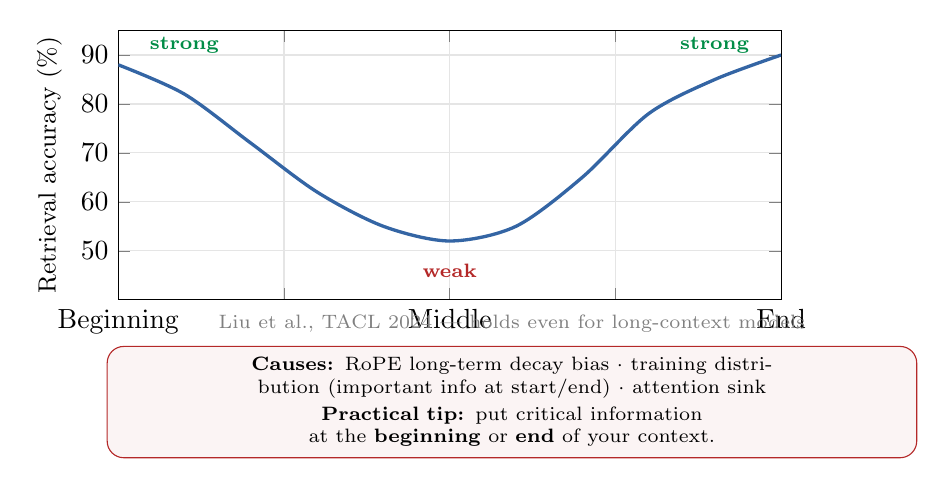
\begin{tikzpicture}
  \begin{axis}[
    width=10cm, height=5cm,
    xlabel={\small Position of relevant information},
    ylabel={\small Retrieval accuracy (\%)},
    xmin=0, xmax=100,
    ymin=40, ymax=95,
    xtick={0, 25, 50, 75, 100},
    xticklabels={Beginning, , Middle, , End},
    ytick={50, 60, 70, 80, 90},
    grid=major,
    grid style={gray!20},
  ]
    % U-shaped curve
    \addplot[very thick, popblue, smooth] coordinates {
      (0, 88) (10, 82) (20, 72) (30, 62) (40, 55)
      (50, 52) (60, 55) (70, 65) (80, 78) (90, 85) (100, 90)
    };

    % Annotations
    \node[font=\scriptsize, text=paramgreen] at (axis cs:10, 92) {\textbf{strong}};
    \node[font=\scriptsize, text=warnred] at (axis cs:50, 46) {\textbf{weak}};
    \node[font=\scriptsize, text=paramgreen] at (axis cs:90, 92) {\textbf{strong}};
  \end{axis}

  % Citation and causes
  \node[font=\scriptsize, text=gray] at (5, -0.3) {Liu et al., TACL 2024 --- holds even for long-context models};

  \node[draw=warnred, fill=warnred!5, rounded corners=6pt, text width=10cm, align=center, inner sep=4pt, font=\scriptsize] at (5, -1.3) {
    \textbf{Causes:} RoPE long-term decay bias $\cdot$ training distribution (important info at start/end) $\cdot$ attention sink\\[2pt]
    \textbf{Practical tip:} put critical information at the \textbf{beginning} or \textbf{end} of your context.
  };
\end{tikzpicture}
\end{center}
\end{frame}

% ============================================================
% NEEDLE IN A HAYSTACK
% ============================================================
\begin{frame}
\frametitle{Needle in a Haystack evaluation}

\begin{center}
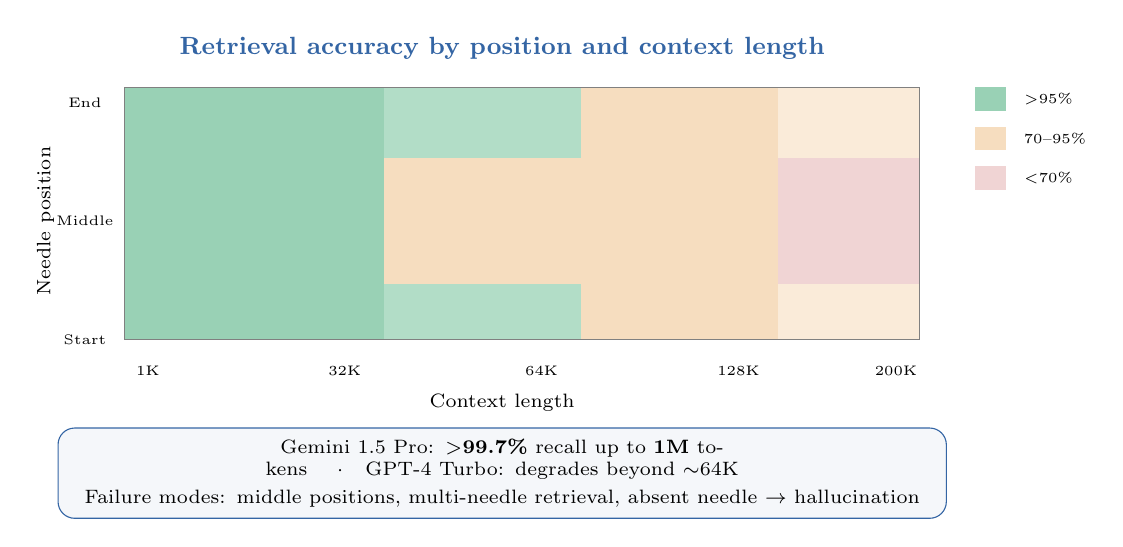
\begin{tikzpicture}
  % Heatmap-style diagram
  \node[font=\small\bfseries, text=popblue] at (0, 3.2) {Retrieval accuracy by position and context length};

  % Y-axis label
  \node[font=\scriptsize, rotate=90] at (-5.8, 1) {Needle position};
  \node[font=\tiny] at (-5.3, 2.5) {End};
  \node[font=\tiny] at (-5.3, 1) {Middle};
  \node[font=\tiny] at (-5.3, -0.5) {Start};

  % X-axis
  \node[font=\scriptsize] at (0, -1.3) {Context length};
  \node[font=\tiny] at (-4.5, -0.9) {1K};
  \node[font=\tiny] at (-2, -0.9) {32K};
  \node[font=\tiny] at (0.5, -0.9) {64K};
  \node[font=\tiny] at (3, -0.9) {128K};
  \node[font=\tiny] at (5, -0.9) {200K};

  % Green (good) regions - short context and edges
  \fill[paramgreen!40] (-4.8, -0.5) rectangle (-1.5, 2.7);
  \fill[paramgreen!30] (-1.5, 1.8) rectangle (1, 2.7);
  \fill[paramgreen!30] (-1.5, -0.5) rectangle (1, 0.2);

  % Yellow (ok) regions
  \fill[orange1!25] (-1.5, 0.2) rectangle (1, 1.8);
  \fill[orange1!25] (1, -0.5) rectangle (3.5, 2.7);

  % Red (poor) regions - long context, middle position
  \fill[warnred!20] (3.5, 0.2) rectangle (5.3, 1.8);
  \fill[orange1!15] (3.5, -0.5) rectangle (5.3, 0.2);
  \fill[orange1!15] (3.5, 1.8) rectangle (5.3, 2.7);

  % Border
  \draw[gray] (-4.8, -0.5) rectangle (5.3, 2.7);

  % Legend
  \fill[paramgreen!40] (6, 2.4) rectangle (6.4, 2.7);
  \node[font=\tiny, right] at (6.5, 2.55) {$>$95\%};
  \fill[orange1!25] (6, 1.9) rectangle (6.4, 2.2);
  \node[font=\tiny, right] at (6.5, 2.05) {70--95\%};
  \fill[warnred!20] (6, 1.4) rectangle (6.4, 1.7);
  \node[font=\tiny, right] at (6.5, 1.55) {$<$70\%};

  % Results table
  \node[draw=popblue, fill=popblue!5, rounded corners=6pt, text width=11cm, align=center, inner sep=4pt, font=\scriptsize] at (0, -2.2) {
    Gemini 1.5 Pro: $>$\textbf{99.7\%} recall up to \textbf{1M} tokens \quad$\cdot$\quad GPT-4 Turbo: degrades beyond $\sim$64K\\[2pt]
    Failure modes: middle positions, multi-needle retrieval, absent needle $\to$ hallucination
  };
\end{tikzpicture}
\end{center}
\end{frame}

% ============================================================
% THE FULL LANDSCAPE
% ============================================================
\begin{frame}
\frametitle{The full landscape}

\begin{center}
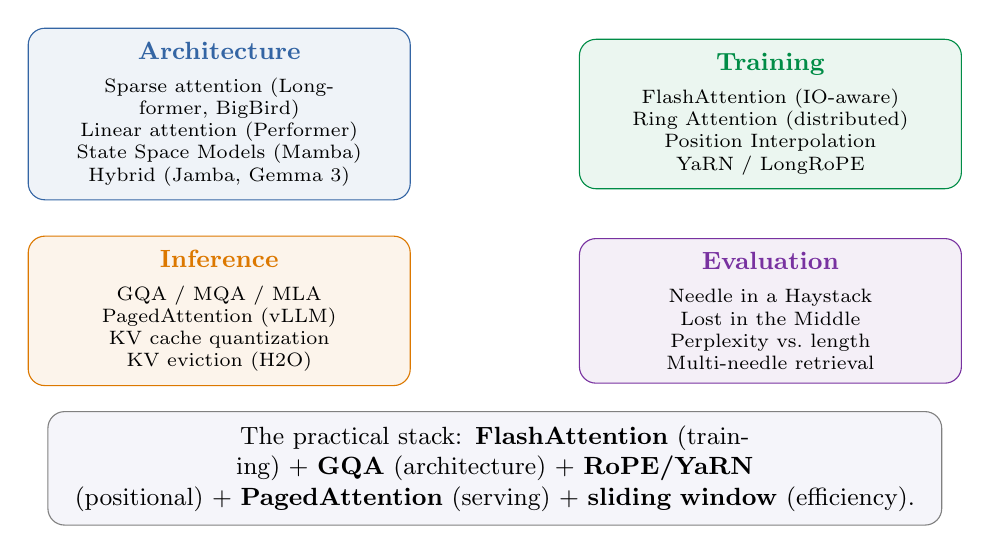
\begin{tikzpicture}
  % Training-time
  \node[draw=popblue, fill=popblue!8, rounded corners=6pt, text width=4.5cm, align=center, inner sep=5pt, font=\scriptsize] at (-3.5, 2.5) {
    {\small\bfseries\textcolor{popblue}{Architecture}}\\[4pt]
    Sparse attention (Longformer, BigBird)\\
    Linear attention (Performer)\\
    State Space Models (Mamba)\\
    Hybrid (Jamba, Gemma 3)
  };

  \node[draw=paramgreen, fill=paramgreen!8, rounded corners=6pt, text width=4.5cm, align=center, inner sep=5pt, font=\scriptsize] at (3.5, 2.5) {
    {\small\bfseries\textcolor{paramgreen}{Training}}\\[4pt]
    FlashAttention (IO-aware)\\
    Ring Attention (distributed)\\
    Position Interpolation\\
    YaRN / LongRoPE
  };

  \node[draw=orange1, fill=orange1!8, rounded corners=6pt, text width=4.5cm, align=center, inner sep=5pt, font=\scriptsize] at (-3.5, 0) {
    {\small\bfseries\textcolor{orange1}{Inference}}\\[4pt]
    GQA / MQA / MLA\\
    PagedAttention (vLLM)\\
    KV cache quantization\\
    KV eviction (H2O)
  };

  \node[draw=violet1, fill=violet1!8, rounded corners=6pt, text width=4.5cm, align=center, inner sep=5pt, font=\scriptsize] at (3.5, 0) {
    {\small\bfseries\textcolor{violet1}{Evaluation}}\\[4pt]
    Needle in a Haystack\\
    Lost in the Middle\\
    Perplexity vs.\ length\\
    Multi-needle retrieval
  };

  % Bottom
  \node[draw=gray, fill=lightbg, rounded corners=6pt, text width=11cm, align=center, inner sep=5pt, font=\small] at (0, -2) {
    The practical stack: \textbf{FlashAttention} (training) + \textbf{GQA} (architecture) + \textbf{RoPE/YaRN}\\
    (positional) + \textbf{PagedAttention} (serving) + \textbf{sliding window} (efficiency).
  };
\end{tikzpicture}
\end{center}
\end{frame}

% ============================================================
% FURTHER READING
% ============================================================
\begin{frame}
\frametitle{Further reading}
\vspace{-0.3cm}
\begin{center}
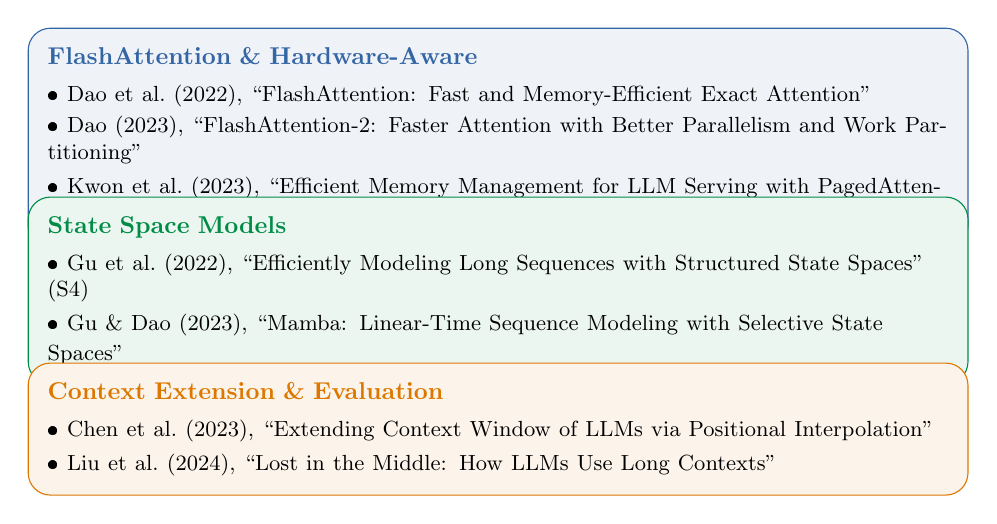
\begin{tikzpicture}[scale=0.88, transform shape]
  \node[draw=popblue, fill=popblue!8, rounded corners=8pt, text width=13cm, align=left, inner sep=8pt] at (0, 2.5) {
    \textbf{\textcolor{popblue}{FlashAttention \& Hardware-Aware}}\\[4pt]
    {\small
    \textbullet~Dao et al.\ (2022), ``FlashAttention: Fast and Memory-Efficient Exact Attention''\\[2pt]
    \textbullet~Dao (2023), ``FlashAttention-2: Faster Attention with Better Parallelism and Work Partitioning''\\[2pt]
    \textbullet~Kwon et al.\ (2023), ``Efficient Memory Management for LLM Serving with PagedAttention'' (vLLM)
    }
  };
  \node[draw=paramgreen, fill=paramgreen!8, rounded corners=8pt, text width=13cm, align=left, inner sep=8pt] at (0, 0.3) {
    \textbf{\textcolor{paramgreen}{State Space Models}}\\[4pt]
    {\small
    \textbullet~Gu et al.\ (2022), ``Efficiently Modeling Long Sequences with Structured State Spaces'' (S4)\\[2pt]
    \textbullet~Gu \& Dao (2023), ``Mamba: Linear-Time Sequence Modeling with Selective State Spaces''
    }
  };
  \node[draw=orange1, fill=orange1!8, rounded corners=8pt, text width=13cm, align=left, inner sep=8pt] at (0, -1.7) {
    \textbf{\textcolor{orange1}{Context Extension \& Evaluation}}\\[4pt]
    {\small
    \textbullet~Chen et al.\ (2023), ``Extending Context Window of LLMs via Positional Interpolation''\\[2pt]
    \textbullet~Liu et al.\ (2024), ``Lost in the Middle: How LLMs Use Long Contexts''
    }
  };
\end{tikzpicture}
\end{center}
\end{frame}

% ============================================================
% QUESTIONS
% ============================================================
\begin{frame}
\begin{center}
\vspace{2cm}
{\Huge \textcolor{popblue}{Questions?}}

\vspace{1cm}
{\normalsize All DL4NLP topics complete!}
\end{center}
\end{frame}

\end{document}
